\documentclass[conference]{IEEEtran}
\IEEEoverridecommandlockouts

\usepackage{cite}
\usepackage{amsmath,amssymb,amsfonts}
\usepackage{algorithmic}
\usepackage{graphicx}
\usepackage{textcomp}
\usepackage{xcolor}
\usepackage{booktabs}
\usepackage{multirow}
\usepackage{array}
\usepackage{url}
\usepackage{tikz}
\usetikzlibrary{arrows.meta, positioning, shapes.geometric, fit, backgrounds, calc}
\usepackage{etoolbox}
\usepackage{placeins}

% Format section and subsection headings to bold
\makeatletter
\patchcmd{\section}{\scshape}{\bfseries\scshape}{}{}
\patchcmd{\subsection}{\itshape}{\bfseries}{}{}
\makeatother

\renewcommand{\thesubsection}{\Alph{subsection}}
\renewcommand{\thesubsectiondis}{\Alph{subsection})}

\def\BibTeX{{\rm B\kern-.05em{\sc i\kern-.025em b}\kern-.08em
    T\kern-.1667em\lower.7ex\hbox{E}\kern-.125emX}}

% Data-derived macros; no desired scores are assigned.
\newcommand{\CurrentFitEngines}{567}
\newcommand{\CurrentSelectionEngines}{36}
\newcommand{\CurrentCalibrationEngines}{35}
\newcommand{\CurrentTestEngines}{71}
\newcommand{\CurrentOfficialEngines}{707}
\newcommand{\CurrentInternalPrefixes}{484}
\newcommand{\CurrentOfficialRMSE}{11.08}
\newcommand{\CurrentInternalRMSE}{12.07}
\newcommand{\CurrentOfficialMAE}{7.19}
\newcommand{\CurrentRegimeCount}{6}
\newcommand{\CurrentGuardCount}{7}
\newcommand{\CurrentNeuralParameters}{353456}
\newcommand{\CurrentRecoveryContexts}{41}
\newcommand{\CurrentBundleHash}{e599e6e25002bec4}
\newcommand{\CurrentLocalLength}{30}
\newcommand{\CurrentGlobalLength}{70}
\newcommand{\CurrentIntactRMSE}{0.02521}
\newcommand{\CurrentCleanFPR}{0.0322}
\newcommand{\CurrentValidationTail}{32.271}
\newcommand{\CurrentBaselineTail}{33.064}
\newcommand{\CurrentRawRMSE}{21.27}
\newcommand{\CurrentLongFraction}{21.2}
\newcommand{\CurrentLongShare}{77.7}
\newcommand{\CurrentPlateauAlpha}{0.000}
\newcommand{\CurrentDetectorParameters}{37909}
\newcommand{\CurrentGeneratorParameters}{176533}
\newcommand{\CurrentPredictorParameters}{136805}
\newcommand{\CurrentCorrectorParameters}{2209}

% Data-derived macros; no desired scores are assigned.
\newcommand{\CurrentNoiseOfficialZero}{11.08}
\newcommand{\CurrentNoiseOfficialTwenty}{11.38}
\newcommand{\CurrentNoiseOfficialFifty}{13.64}
\newcommand{\CurrentNoiseHeldoutZero}{12.07}
\newcommand{\CurrentNoiseHeldoutFifty}{14.36}
\newcommand{\CurrentNoiseCoverageTwenty}{98.6}
\newcommand{\CurrentNoiseCoverageFifty}{97.0}
\newcommand{\CurrentNoiseDropoutTwo}{10.94}
\newcommand{\CurrentNoiseDropoutFive}{11.10}
\newcommand{\CurrentPaperAOursFdA}{10.13}
\newcommand{\CurrentPaperAFdA}{13.1}
\newcommand{\CurrentPaperBOfficial}{12.15}
\newcommand{\CurrentBestFdA}{10.61}
\newcommand{\CurrentBestFdB}{10.71}
\newcommand{\CurrentRankFdA}{1}
\newcommand{\CurrentRankFdB}{1}

% Data-derived macros; no desired scores are assigned.
\newcommand{\CurrentAblationCleanFull}{11.08}
\newcommand{\CurrentAblationCleanPlain}{10.95}
\newcommand{\CurrentAblationStuckFull}{12.11}
\newcommand{\CurrentAblationStuckBypass}{22.58}
\newcommand{\CurrentAblationStuckGain}{10.47}
\newcommand{\CurrentAblationStuckGainLow}{9.06}
\newcommand{\CurrentAblationStuckGainHigh}{10.78}
\newcommand{\CurrentAblationMixedGain}{3.17}
\newcommand{\CurrentAblationOutageGain}{1.26}
\newcommand{\CurrentAblationBlockGain}{0.49}
\newcommand{\CurrentAblationNoiseGain}{0.14}
\newcommand{\CurrentAblationCorrectorDelta}{0.00}
\newcommand{\CurrentAblationWidth}{60.3}
\newcommand{\CurrentAblationCoverage}{98.4}

% Data-derived macros; no desired scores are assigned.
\newcommand{\CurrentParams}{348,976}
\newcommand{\CurrentParamMB}{1.33}
\newcommand{\CurrentLatency}{5.4}
\newcommand{\CurrentThroughput}{10184}
\newcommand{\CurrentIntactWorst}{0.020}
\newcommand{\CurrentFalseRepairWorst}{0.5}
\newcommand{\CurrentRecallLowest}{0.27}


\begin{document}

\title{Auditable Remaining Useful Life Prediction Under Correlated Sensor Failures: Guarded Recovery for Turbofan Engines\\
\thanks{This manuscript presents an auditable prognostic pipeline and an empirical evaluation on reference and structured sensor-fault NASA C-MAPSS telemetry, including observed recovery limitations and an explicit failure analysis.}
}

\author{\IEEEauthorblockN{Devanshu Verma}
\IEEEauthorblockA{\textit{Department of DSAI} \\
\textit{IIIT-Naya Raipur}\\
Email: devanshu24102@iiitnr.edu.in}
\and
\IEEEauthorblockN{Devesh Gour}
\IEEEauthorblockA{\textit{Department of DSAI} \\
\textit{IIIT-Naya Raipur}\\
Email: devesh24102@iiitnr.edu.in}
\and
\IEEEauthorblockN{Vishal Agrawal}
\IEEEauthorblockA{\textit{Department of DSAI} \\
\textit{IIIT-Naya Raipur}\\
Email: vishal24102@iiitnr.edu.in}
}

\maketitle

\begin{abstract}
Remaining useful life (RUL) prediction must distinguish degradation from measurement failures across operating conditions. GRACE-RUL combines local CNN--GRU features, residual BiLSTM sensor recovery, Transformer context, an independent finite-fault detector and a validation-audited RUL path. Format 10 adds an observed engine-age channel and supervises continuity on the deployed repair path; it disables the bounded corrector after a null component ablation and replaces the hard repair threshold with probability-weighted soft gating. One shared model pools all four NASA C-MAPSS subsets with 567 fitting, 36 selection, 35 calibration and 71 internal-test engines. Faults follow related-channel, temporally persistent mechanisms in raw sensor units. Conservative thresholds, fitting-only support bounds and a complete 41-condition audit limit healthy-sensor displacement, while detector recall remains low on drift, bias and noise. Predictor refinement uses active-path paired-prefix continuity, fitting-error tails and corruption-aware RUL supervision. A validation-selected candidate is frozen before interval calibration and test evaluation. On 707 official endpoints its capped RMSE is 11.08 cycles, MAE is 7.19, and severity-0.2 stuck-fault RMSE averages 12.11 over three corruption replicates. Internal clean RMSE is 12.07 over 484 prefixes from 71 engines. Observable interval scales are fitted independently of engine-level conformal calibration. Raw RMSE is 21.27; 150 engines with raw RUL above 125 account for 77.7\% of raw squared error. The monotone plateau stretch was available, but its non-increasing capped-RMSE guard rejected every positive value (alpha=0), so the raw-target bias is not reduced. A previously inspected severe prediction failure is reported explicitly. Under broadband sensor noise at 20\% of the within-regime scale, capped RMSE rises from \CurrentNoiseOfficialZero{} to \CurrentNoiseOfficialTwenty{} cycles with \CurrentNoiseCoverageTwenty{}\% empirical coverage; at 50\% it is \CurrentNoiseOfficialFifty{} cycles. Reused benchmarks, one training seed and simulated faults limit generalization claims.

\end{abstract}
\begin{IEEEkeywords}
Remaining useful life, C-MAPSS, correlated sensor faults, guarded recovery, pooled training, CNN--GRU, Transformer, conformal calibration.
\end{IEEEkeywords}
% Generated from hashed saved numerical evidence.

\newcommand{\CurrentPartitionTable}{%
\begin{table*}[!t]
\caption{Format-10 pooled engine-disjoint data partitions.}
\label{tab:pooled_partitions}
\centering\footnotesize
\setlength{\tabcolsep}{3pt}
\begin{tabular}{lrrrrrr}
\toprule
Subset & Available training & Fit & Selection & Calibration & Internal test & Official test \\
\midrule
FD001 & 100 & 80 & 5 & 5 & 10 & 100 \\
FD002 & 260 & 208 & 13 & 13 & 26 & 259 \\
FD003 & 100 & 80 & 5 & 5 & 10 & 100 \\
FD004 & 249 & 199 & 13 & 12 & 25 & 248 \\
\bottomrule
\end{tabular}
\par\vspace{2pt}
\begin{minipage}{\textwidth}\scriptsize The 10\% development pool is divided equally between selection and independent calibration; integer rounding gives the exact counts above. Internal observations are fixed-grid prefixes, not independent engines. Official test engines are read only after the candidate and calibration are frozen.\end{minipage}
\end{table*}
}

\newcommand{\CurrentPooledResultsTable}{%
\begin{table*}[!t]
\caption{Format-10 model: capped-target clean and structured-fault results.}
\label{tab:current_pooled}
\centering\footnotesize
\setlength{\tabcolsep}{3pt}
\begin{tabular}{lrrrrrrrr}
\toprule
Subset & $N_{\rm off}$ & RMSE & MAE & NASA $S$ & Cov. (\%) & Stuck & Mixed & Internal RMSE \\
\midrule
POOLED & 707 & 10.50 & 6.96 & 1433.1 & 99.7 & 12.49 & 11.48 & 11.80 \\
FD001 & 100 & 10.04 & 7.31 & 156.3 & 100.0 & 11.41 & 11.42 & 8.75 \\
FD002 & 259 & 10.92 & 7.20 & 530.8 & 99.6 & 12.53 & 12.02 & 9.99 \\
FD003 & 100 & 9.35 & 6.03 & 186.5 & 100.0 & 10.94 & 10.00 & 7.59 \\
FD004 & 248 & 10.67 & 6.95 & 559.6 & 99.6 & 13.40 & 11.45 & 15.26 \\
\bottomrule
\end{tabular}
\par\vspace{2pt}
\begin{minipage}{\textwidth}\scriptsize Fault columns average three corruption replicates at severity 0.2; these are not training-seed replications. Coverage is empirical clean prefix/endpoint coverage. Internal RMSE uses all saved prefixes from each source's reserved engines. Targets are $\min(r,125)$; units are cycles except NASA score and coverage.\end{minipage}
\end{table*}
}

\newcommand{\CurrentComparisonTable}{%
\begin{table*}[!t]
\caption{Pooled comparison with the preserved v9 source.}
\label{tab:current_comparison}
\centering\footnotesize
\setlength{\tabcolsep}{3pt}
\begin{tabular}{lrrr}
\toprule
Artifact & Official clean RMSE & Internal clean RMSE & Stuck @0.2 \\
\midrule
Original revision 2 & 12.106 & 13.441 & 18.858 \\
Preserved v9 source & 12.008 & 13.297 & 15.077 \\
Format-10 repair & 10.496 & 11.797 & 12.489 \\
\bottomrule
\end{tabular}
\par\vspace{2pt}
\begin{minipage}{\textwidth}\scriptsize All rows use their own saved predictions and capped targets. The stuck column uses the common severity-0.2 setting over three corruption realizations; higher-severity v9 values are not mixed in because the format-10 official evaluation was run at severity 0.2 only. The held selection recovery audit still covers all declared severities. v9 test values are reused descriptive evidence and did not select the format-10 candidate.\end{minipage}
\end{table*}
}

\newcommand{\CurrentRawResultsTable}{%
\begin{table*}[!t]
\caption{Clean official results against original, uncapped RUL.}
\label{tab:current_raw}
\centering\footnotesize
\setlength{\tabcolsep}{3pt}
\begin{tabular}{lrrrr}
\toprule
Subset & Raw RMSE & Raw MAE & Raw NASA $S$ & Raw coverage (\%) \\
\midrule
POOLED & 20.47 & 12.98 & 7229.2 & 99.7 \\
FD001 & 11.33 & 8.35 & 181.9 & 100.0 \\
FD002 & 23.09 & 14.62 & 3826.6 & 99.6 \\
FD003 & 10.90 & 7.51 & 214.4 & 100.0 \\
FD004 & 23.18 & 15.35 & 3006.3 & 99.6 \\
\bottomrule
\end{tabular}
\par\vspace{2pt}
\begin{minipage}{\textwidth}\scriptsize The point model is trained on capped targets. A monotone plateau stretch was evaluated on held selection engines but was not applied because no positive value respected the non-increasing capped-RMSE guard. Raw errors therefore expose the censoring limitation rather than a solved long-horizon task. Raw coverage uses separately calibrated intervals and must not be read as capped-target coverage.\end{minipage}
\end{table*}
}

\newcommand{\CurrentAdaptiveCalibrationTable}{%
\begin{table*}[!t]
\caption{Observable interval scales and radii of the frozen format-10 model.}
\label{tab:adaptive_calibration}
\centering\footnotesize
\setlength{\tabcolsep}{3pt}
\begin{tabular}{lrrrrr}
\toprule
Predicted RUL bin & Scale capped & Scale raw & Radius capped & Radius raw & Scale engines \\
\midrule
$[0,35)$ & 3.97 & 3.97 & 22.38 & 17.01 & 36 \\
$[35,75)$ & 6.82 & 6.82 & 38.48 & 29.25 & 36 \\
$[75,125)$ & 11.20 & 46.48 & 63.21 & 199.39 & 36 \\
$[125,\infty)$ & 4.21 & 123.15 & 23.74 & 528.28 & 36 \\
\bottomrule
\end{tabular}
\par\vspace{2pt}
\begin{minipage}{\textwidth}\scriptsize Scales use selection engines only. A single engine-maximum normalized score spans all bins and is calibrated on 35 separate engines; alpha=0.1, rank=33. Scale-engine counts are overlapping bin support, not independent calibration sample counts. No true RUL is required to choose a bin at inference.\end{minipage}
\end{table*}
}

\newcommand{\CurrentLongRULTable}{%
\begin{table*}[!t]
\caption{Clean official long-horizon behaviour.}
\label{tab:current_long}
\centering\footnotesize
\setlength{\tabcolsep}{3pt}
\begin{tabular}{lr}
\toprule
Quantity & Value \\
\midrule
Raw RMSE (cycles) & 20.47 \\
Capped RMSE (cycles) & 10.50 \\
Engines with raw RUL $>125$ & 150/707 (21.2\%) \\
Long-engine mean prediction & 120.00 \\
Long-engine mean target & 154.07 \\
Long-engine share of raw squared error & 77.5\% \\
Worst engine maximum absolute error & 84.27 \\
Engines with max error $>40$ cycles & 56/707 \\
\bottomrule
\end{tabular}
\par\vspace{2pt}
\begin{minipage}{\textwidth}\scriptsize Plateau stretch $\alpha=0.150$ above 105 cycles, selected on held validation engines under a non-increasing capped-RMSE guard; $\alpha=0$ means the guard rejected every positive stretch. Engine bootstrap 95\% intervals for capped RMSE are [9.71, 11.31] and for raw RMSE [19.11, 21.86] (whole-engine resampling). Any positive stretch is monotone but cannot recover an individual engine's unknown censored target.\end{minipage}
\end{table*}
}

\newcommand{\CurrentIntervalBandTable}{%
\begin{table*}[!t]
\caption{Clean official coverage and width by observable RUL band.}
\label{tab:interval_bands}
\centering\footnotesize
\setlength{\tabcolsep}{3pt}
\begin{tabular}{lrrrrr}
\toprule
Raw-RUL band & $N$ & Capped cov. (\%) & Capped width & Raw cov. (\%) & Raw width \\
\midrule
0--35 & 171 & 100.0 & 38.7 & 100.0 & 31.3 \\
35--75 & 144 & 100.0 & 81.3 & 100.0 & 86.2 \\
75--125 & 242 & 99.2 & 119.2 & 99.2 & 287.9 \\
$\geq125$ & 150 & 100.0 & 107.5 & 100.0 & 398.3 \\
\bottomrule
\end{tabular}
\par\vspace{2pt}
\begin{minipage}{\textwidth}\scriptsize Bands are chosen from the raw target for description only; inference uses the predicted-RUL bin. Coverage is marginal over engines and prefixes, not conditional on a realized engine. Raw width can be unbounded; mean widths include finite values only and are descriptive.\end{minipage}
\end{table*}
}

\raggedbottom

\section{\textbf{Introduction}}
Turbofan RUL estimation maps observed operating history to remaining cycles before
failure. Missing sensor readings are observable, while a finite bias, drift or
stuck reading can resemble degradation. Operating-condition changes make this
distinction harder. C-MAPSS provides a reproducible simulation benchmark, but
added measurement faults are modeling assumptions rather than recorded aircraft
incidents~\cite{saxena2008damage}.

GRACE-RUL is organized around three design commitments: local
convolutional--recurrent modeling of recent degradation, selective recurrent
recovery of corrupted readings, and a Transformer context branch. The current
format-10 implementation adds an observed engine-age
channel and a probability-weighted finite-repair gate to one shared model across
FD001--FD004, without requiring a subset label at deployment. Its contributions
are a prefix-consistent related-channel fault simulator; independent finite-fault
detection with soft, support-bounded repair; quality-conditioned local/global
RUL fusion; validation-led predictor refinement; independently calibrated
observable intervals; and a broadband measurement-noise and channel-dropout
benchmark that reports accuracy and calibrated coverage without refitting.
Complete recovery checks and state-bound audits make the selected path
inspectable. Severe prediction failures, reused benchmarks and unvalidated fleet
assumptions are retained explicitly in the evidence.

\section{\textbf{Related Work}}
\label{sec:related_work}
\subsection{\textbf{Local Degradation Modeling and Interpretation}}
The supplied hybrid CNN--GRU study emphasizes local feature extraction, temporal degradation modeling, and sensor-level interpretation \cite{ozupak2026hybrid}. GRACE-RUL retains a CNN--GRU branch over the most recent 30 cycles. Interpretation is implemented as optional post-training KernelSHAP/LIME analysis \cite{lundberg2017unified,ribeiro2016trust}; it is not a term in the neural training objective. That work's complete reliability/generalization/explainability formulation is not reproduced literally.

\subsection{\textbf{Recovery Under Partial Sensor Failure}}
The partial-failure study motivates paired corrupted/reference histories, bidirectional recurrent recovery, and a training-only adversarial critic \cite{tang2026deep}. The implementation adds a deployment-available finite-fault detector and availability-based selective blending, because synthetic altered-entry labels are unavailable at inference. WGAN-GP supplies the adversarial training objective \cite{gulrajani2017improved}. Original C-MAPSS readings remain noisy reference measurements, rather than pristine sensor truth.

\subsection{\textbf{Transformer Context and Residual Compensation}}
Trans-D3 motivates combining a Transformer representation with prediction correction \cite{paredes2026trans}. The current implementation instead uses a bounded supervised residual MLP only as a retained, zero-bound ablation artifact; after a null component ablation it is disabled in the deployed format-10 path, so the final RUL is the branch-fusion base prediction. The study also uses physical degradation slew and anti-rebound loss penalties on paired engine prefixes. It contains no TD3 actor, twin action-value critics, replay buffer, policy update, or LQR filter. The separate WGAN critic evaluates sensor sequences during recovery training and is unrelated to reinforcement learning.

\section{\textbf{Problem Statement and Data Protocol}}
\label{sec:problem_statement}
\subsection{\textbf{Observed Histories, Targets and Masks}}
An observation contains three operating settings and 21 sensors. Engine ID is
never a neural feature; the observed cycle index is used only to derive the
normalized age channel in format 10. A window ending at $t$
contains at most $L=\CurrentGlobalLength$ already observed cycles, left-padded to
fixed length. Validity $V$ masks padding and availability $M$ marks finite sensor
readings. Normalized settings are $U$ and encoded observed sensors are $S$;
nonfinite measurements are replaced by zero after the mask is constructed. A
zero measurement remains valid.
For a complete fitting engine ending at $T_e$, raw RUL is $r_{e,t}=T_e-t$ and
\begin{equation}y_{e,t}=\min(125,r_{e,t}).\label{eq:rul_target}\end{equation}
Official RUL labels enter evaluation after freeze. Targets, future observations,
source identity and simulated altered-entry labels never enter inference.
Softplus estimates may exceed 125: the cap specifies the target, not a hard
prediction ceiling or a guarantee about future failure time.

\subsection{\textbf{One Pooled Engine-Disjoint Split}}
\CurrentPartitionTable
The available four training files are pooled after namespacing engine IDs for
bookkeeping. Split seed 42 assigns approximately 80\% to fitting, 10\% to a
selection/calibration pool and 10\% to internal test. Half of the development
pool is reserved for independent interval calibration. Exact rounded counts are
\CurrentFitEngines{} fitting, \CurrentSelectionEngines{} selection,
\CurrentCalibrationEngines{} calibration and \CurrentTestEngines{} internal-test
engines. Every prefix of an engine stays in its partition. Per-FD reporting is
an evaluation breakdown, not a collection of different models.

\subsection{\textbf{Fitting-Only Regimes and Encoding}}
Operating settings are standardized using fitting engines only. GMM BIC selects
the regime count from fitting settings, followed by K-means assignment; the
selected shared scaler has \CurrentRegimeCount{} regimes. Per-regime sensor
means/scales include measurement-resolution floors. For raw sensor $x_j$ in
assigned regime $k$,
\begin{align}
 z_j&=(x_j-\mu_{kj})/\sigma_{kj},\\
 e_j&=s\operatorname{asinh}(z_j/s),\qquad s=1,\\
 \phi^{-1}(e_j)&=s\sinh(e_j/s).
 \label{eq:encoding}
\end{align}
This invertible encoding compresses extreme standardized values; it does not
reduce their physical raw-unit error. Faults are applied after decoding and only
changed cells are re-encoded. Intact encoded cells retain their bits. Recovery
support is the empirical per-regime/channel fitting range, not a certified
manufacturer operating envelope. Selection, calibration and test engines fit
none of these statistics.

\subsection{\textbf{Causal Prefix Evaluation}}
Fitting uses engine-balanced sampling from eligible within-engine windows.
Selection and internal testing use a fixed inspection grid, beginning at cycle
30 with stride 30, independent of eventual failure. Calibration evaluates every
observed prefix of each reserved complete engine. Official test evaluation uses
its final observed endpoint. Bidirectional recovery and non-triangular attention
operate inside the already observed window; unseen future readings are absent.
The local branch uses \CurrentLocalLength{} cycles and the global branch
\CurrentGlobalLength{}. Neither enforces monotonic predictions at inference.

\subsection{\textbf{Data Integrity and Evidence Boundaries}}
The shared model receives only normalized operating settings, observed sensors,
availability and the observed-history mask. Engine IDs, subset labels, future
readings, true RUL and simulated altered-entry masks are excluded from inference.
Related-channel fault histories are prefix-consistent: appending future rows does
not alter an earlier corruption realization or select onset by eventual failure.

The four original training files define the engine-disjoint fit/selection/
calibration/internal-test groups in Table~\ref{tab:pooled_partitions}. Scaler,
raw-unit fault scales and repair support use fitting engines only. Fitting-engine
OOF features were used to train the source corrector and exclude their held fold
from temporary fitting and inner selection; in format 10 that corrector is
disabled with a zero bound and contributes no inference feature or adjustment.
Predictor refinement uses fitting engines; every clean/source/NASA, mixed/stuck
and tail-selection check uses held selection engines. Calibration engines enter
only after that choice is fixed.

New artifacts use fresh directories and retain their source SHA-256. Resuming an
interrupted refinement requires matching source, recipe and implementation.
Current detector audits bind the actual deployed thresholds and detector state;
the earlier detector operating point remains historical metadata. Recovery
proofs bind the full declared context matrix, selection IDs and sensor-repair
state. Calibration binds the final model/configuration and its separate scale
scope. Strict reload rejects stale or mismatched records.

Validation-only development runs block official test/RUL and saved test-result
reads. These checks document within-run separation. Earlier internal and
official test cases have already informed development; their later evaluation
remains exploratory and is not an untouched independent generalization test.


\section{\textbf{Structured Sensor and Acquisition Faults}}
\label{sec:faults}
Added corruption models measurement failure while retaining original degradation and RUL labels. A profile selects a related measurement domain: temperature, pressure, fan speed, core speed, coolant flow, or an individual derived quantity. These groupings are measurement-based assumptions, not verified wiring diagrams. Operating settings and the two speed-demand columns are preserved.

\begin{table}[!t]
\caption{Implemented fault mechanisms. Severity is not a missing-cell percentage.}
\label{tab:fault_mechanisms}
\centering\footnotesize
\begin{tabular}{p{0.19\columnwidth}p{0.70\columnwidth}}
\toprule Family & Temporal and channel structure\\\midrule
Intermittent & Related-channel burst dropout; minimum two cycles, configured mean four.\\
Outage & Persistent channel unavailability after onset.\\
Block & Recurring missing blocks with intact gaps of 25--50 cycles by default.\\
Noise & AR(1) error, $\rho=0.9$; common-source and individual innovation variance weights 0.8/0.2.\\
Bias & Persistent additive calibration offset in raw sensor units.\\
Drift & Raw-unit offset ramps over 100 cycles to its bounded level.\\
Stuck & A physical reading freezes at onset, including across regime transitions.\\
Mixed & Connector: noise/intermittent; calibration: bias/drift; acquisition: stuck/block.\\\bottomrule
\end{tabular}
\end{table}

Mixed mechanisms share a domain, channels, and onset. Regime transitions causally increase noise amplitude and burst-entry risk through a stress proxy computed from already observed settings. Bias/drift bounds scale with $2.5v$ times the fitting fault scale; noise amplitude also depends on $v$. Onset is an observed offset between zero and 100 cycles, independent of eventual failure time. Seeded streams preserve prefixes when future rows are appended, and cached histories give overlapping windows identical corruption.

Randomness represents uncertain occurrence within a specified fault process. It is temporally and physically structured rather than independent arbitrary perturbation of every entry. Training samples $v\in\{0.1,0.2,0.3\}$ with a ten-epoch curriculum. The default clean-realization probability is 0.25, not a batch quota. The historical format-5 study used selected subset overrides. Severities 0.4 and 0.5 extend beyond the default sampled training levels. A stuck reading can generate a large error after a regime transition even at $v=0.2$. No severity parameter has been calibrated to field failure rates.

\section{\textbf{Current Framework Architecture}}
\label{sec:architecture}
Fig.~\ref{fig:architecture} separates inference from training-only supervision. A single pooled parameter set serves all four source subsets; operating settings condition the computation. The recovery guard adds fitting-only buffers and a deterministic projection.

\subsection{\textbf{Independent Finite-Fault Detector}}
The detector receives $[S,M,U]$ (45 features per cycle). Parallel kernel-three and kernel-five convolutions each produce 32 ReLU channels. A GRU-64 and linear 21-logit head yield sigmoid discrimination scores $p$. The head starts with zero weights and bias $-4$, so its initial score is approximately 0.018. A constant initialized head is not reported as learned fault evidence.

Only finite, real entries train the classifier. For each sensor, binary cross entropy is averaged separately over present altered and intact classes, those present-class means are averaged, and sensor losses are then averaged. Missing readings do not become finite-fault positives. The detector is fitted independently on fitting engines using clean and all fault/mixed contexts. Validation selects its checkpoint and representable sensor thresholds $\tau_j$, subject to at most 5\% empirical intact false positives in each validation channel/context. Scores are not calibrated physical failure probabilities.

The format-10 deployed gate uses $p_j^3$ as a continuous finite-repair weight rather than a binary threshold crossing, with $\tau_j=1$ as the only hard channel disable. The cubic power was fixed by a held-validation sweep: power 1.0 failed the FD003 noise recovery guard, whereas power 3.0 preserved it while improving clean and stuck validation. This soft gate mitigates, but does not remove, the low-recall failure mode.

The deployed threshold vector starts from a conservative floor and tightens only
channels that violate a source/context false-positive bound on held selection
engines; under the soft gate it acts only as the channel-disable mask. Its
current audit binds the actual thresholds and detector state; previous detector
metrics remain explicitly historical. The detector is frozen during generator,
joint and predictor-refinement training. Detached scores drive the generator and
recovery gates, so RUL/reconstruction gradients cannot redefine fault
classification. Threshold $\tau_j=1$ explicitly disables finite repair, including
when sigmoid rounds to one.

\subsection{\textbf{Residual Generation and Soft Proposal}}
A two-layer bidirectional LSTM with hidden size 64 per direction receives $[S,M,p,U]$ (66 features). A $128\rightarrow64\rightarrow21$ ReLU decoder, initialized with a zero final layer, produces
\begin{align}
 G&=S+f_{\mathrm{BiLSTM}}([S,M,\operatorname{sg}(p),U]),\\
 \bar p_j&=\operatorname{sg}(p_j)^{3}\,\mathbf{1}\{\tau_j<1\},\\
 W&=(1-M)+M\odot\bar p,\\
 R^\star&=(1-W)\odot S+W\odot G.
 \label{eq:recovery}
\end{align}
Here $\operatorname{sg}$ stops gradients. Missing entries route to $G$; finite readings are weighted continuously by the cubic detector score, with $\tau_j=1$ as the only hard channel disable. The generator residual is unconstrained internally, but the deployed finite proposal is subsequently bounded. A bypass sets $R=S$ and supplies zero recovery weights to the predictor. All stages exclude padding.

\subsection{\textbf{Fitting-Support Guard for Finite Readings}}
Let $x=\phi^{-1}(S_j)$ be a finite observed standardized reading, and let $[\ell,u]$ be its fitting support in the selected regime. With existing displacement budget $\varepsilon=0.15$, define
\begin{equation}
 \mathcal{I}(x;\ell,u)=
 \begin{cases}
 [x-\varepsilon,x+\varepsilon],&\ell\leq x\leq u,\\
 [\ell-\varepsilon,x+\varepsilon],&x>u,\\
 [x-\varepsilon,u+\varepsilon],&x<\ell.
 \end{cases}
 \label{eq:support_interval}
\end{equation}
The finite result is
\begin{equation}
 R_j=\phi\!\left(\operatorname{clip}
   (\phi^{-1}(R_j^\star),\mathcal{I}(x;\ell,u))\right).
 \label{eq:support_projection}
\end{equation}
Bounds round inward to representable values, preserving identity proposals. An observed inlier therefore moves at most $\varepsilon$ in original-linear standardized coordinates. An outlier may return throughout the fitting range in one step; outward movement remains budgeted. Missing imputation is unchanged. Projection uses ordinary clamp gradients without a straight-through estimator.

This is a conditional guarantee about an observed inlier, including a genuinely corrupted reading that happens to lie inside the support. It can restrict useful small-fault correction. A healthy unseen reading can lie outside fitting support and receive a larger inward move. Thus the rule is neither a universal healthy-cell guarantee nor a raw-unit tolerance of 0.15. Raw displacement depends on $\sigma_{kj}$.

% Shared format-9 inference architecture; native IEEE figure.
\begin{figure*}[!t]
\centering
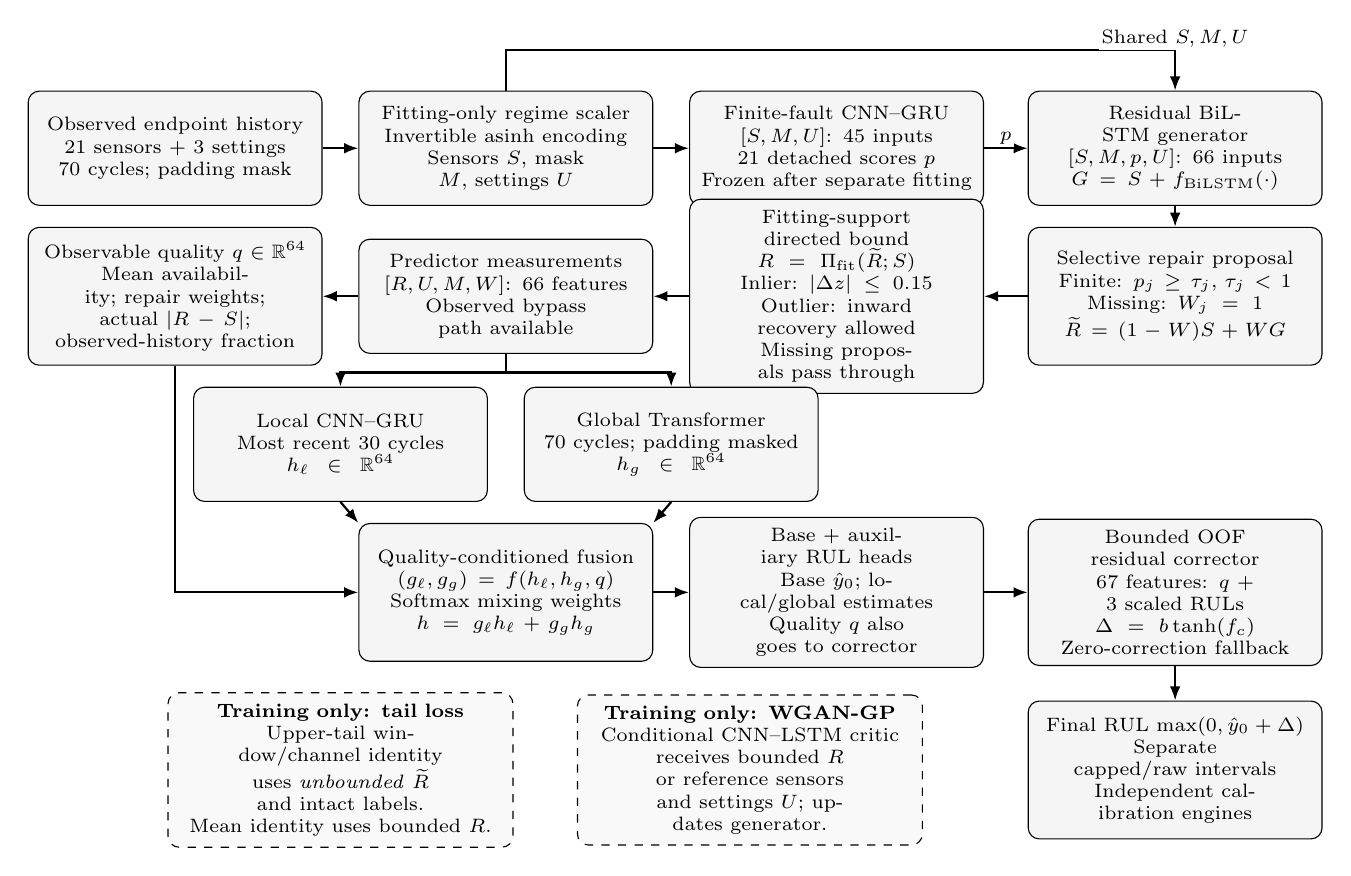
\begin{tikzpicture}[y=.94cm,
 box/.style={draw,rounded corners,fill=gray!8,align=center,text width=3.45cm,minimum height=1.45cm,inner sep=4pt,font=\scriptsize},
 train/.style={box,dashed,fill=gray!5,text width=4.10cm,minimum height=1.85cm},
 link/.style={-{Latex[length=1.8mm]},thick},
 note/.style={font=\scriptsize,align=center,fill=white,inner sep=1pt}]
\node[box] (history) at (1.8,0) {Observed endpoint history\\21 sensors + 3 settings\\70 cycles; padding mask};
\node[box] (scale) at (6.0,0) {Fitting-only regime scaler\\Invertible asinh encoding\\Sensors $S$, mask $M$, settings $U$};
\node[box] (detect) at (10.2,0) {Finite-fault CNN--GRU\\$[S,M,U]$: 45 inputs\\21 detached scores $p$\\Frozen after separate fitting};
\node[box] (generator) at (14.5,0) {Residual BiLSTM generator\\$[S,M,p,U]$: 66 inputs\\$G=S+f_{\rm BiLSTM}(\cdot)$};
\draw[link] (history)--(scale);
\draw[link] (scale)--(detect);
\draw[link] (detect)-- node[note,above] {$p$} (generator);
\draw[link] (scale.north)--++(0,.55)-| node[note,pos=.52,above] {Shared $S,M,U$} (generator.north);

\node[box,minimum height=1.75cm] (blend) at (14.5,-2.0) {Selective repair proposal\\Finite: $p_j\geq\tau_j$, $\tau_j<1$\\Missing: $W_j=1$\\$\widetilde R=(1-W)S+WG$};
\node[box,minimum height=1.85cm] (bound) at (10.2,-2.0) {Fitting-support directed bound\\$R=\Pi_{\rm fit}(\widetilde R;S)$\\Inlier: $|\Delta z|\leq0.15$\\Outlier: inward recovery allowed\\Missing proposals pass through};
\node[box] (features) at (6.0,-2.0) {Predictor measurements\\$[R,U,M,W]$: 66 features\\Observed bypass path available};
\node[box,minimum height=1.75cm] (quality) at (1.8,-2.0) {Observable quality $q\in\mathbb R^{64}$\\Mean availability; repair weights;\\actual $|R-S|$;\\observed-history fraction};
\draw[link] (generator)--(blend);
\draw[link] (blend)--(bound);
\draw[link] (bound)--(features);
\draw[link] (features)--(quality);

\node[box] (local) at (3.9,-4.0) {Local CNN--GRU\\Most recent 30 cycles\\$h_\ell\in\mathbb R^{64}$};
\node[box] (global) at (8.1,-4.0) {Global Transformer\\70 cycles; padding masked\\$h_g\in\mathbb R^{64}$};
\draw[link] (features.south)--++(0,-.25)-| (local.north);
\draw[link] (features.south)--++(0,-.25)-| (global.north);
\node[box,minimum height=1.75cm] (fusion) at (6.0,-6.0) {Quality-conditioned fusion\\$(g_\ell,g_g)=f(h_\ell,h_g,q)$\\Softmax mixing weights\\$h=g_\ell h_\ell+g_g h_g$};
\node[box,minimum height=1.75cm] (heads) at (10.2,-6.0) {Base + auxiliary RUL heads\\Base $\hat y_0$; local/global estimates\\Quality $q$ also goes to corrector};
\node[box,minimum height=1.75cm] (corrector) at (14.5,-6.0) {Bounded OOF residual corrector\\67 features: $q$ + 3 scaled RULs\\$\Delta=b\tanh(f_c)$\\Zero-correction fallback};
\draw[link] (local.south)--(fusion.north west);
\draw[link] (global.south)--(fusion.north east);
\draw[link] (quality.south)|-(fusion.west);
\draw[link] (fusion)--(heads);
\draw[link] (heads)--(corrector);

\node[train] (tail) at (3.9,-8.4) {\textbf{Training only: tail loss}\\Upper-tail window/channel identity\\uses \emph{unbounded} $\widetilde R$ and intact labels.\\Mean identity uses bounded $R$.};
\node[train] (critic) at (9.1,-8.4) {\textbf{Training only: WGAN-GP}\\Conditional CNN--LSTM critic\\receives bounded $R$ or reference sensors\\and settings $U$; updates generator.};
\node[box,minimum height=1.75cm] (output) at (14.5,-8.4) {Final RUL $\max(0,\hat y_0+\Delta)$\\Separate capped/raw intervals\\Independent calibration engines};
\draw[link] (corrector)--(output);
\end{tikzpicture}
\caption{Shared format-9 computation for every source subset; a subset label is not an inference input. The directed bound acts in original, uncompressed regime-standardized sensor coordinates $z$, using fitting-only support. The 0.15 budget applies to observations inside that support; large outliers can move inward without a universal small-step cap. The detector and generator remain frozen during the reported predictor refinement. Dashed components describe source recovery training, and the WGAN critic is absent at deployment. Deterministic paired-prefix and fitting-tail objectives refine the predictor without adding a hard inference floor or monotonic constraint. Altered-entry labels and targets never enter deployment.}
\label{fig:architecture}
\end{figure*}


\subsection{\textbf{Local and Global Prognostic Branches}}
The predictor receives $[R,U,M,W]$ (66 features) together with one normalized observed-cycle age channel (67 features in format 10). Its local branch uses the last 30 cycles: parallel kernel-three/five convolutions with 32 channels each, GRU-64, and a $64\rightarrow64$ last-valid-output projection. Repaired local values may depend on the entire observed recovery window. The global branch projects the 70-cycle input to 64 dimensions, adds sinusoidal positions, and uses two Transformer encoder layers with four heads, feed-forward width 128, GELU and dropout 0.2. Padding is masked; the last valid token represents global context.

\subsection{\textbf{Quality Fusion and RUL Heads}}
The quality vector $q\in\mathbb{R}^{64}$ concatenates time-mean availability (21), recovery weights (21), absolute actual changes $|R-S|$ (21), and observed-history fraction (one). A $192\rightarrow32\rightarrow2$ gate combines local and global features:
\begin{align}
 (g_\ell,g_g)&=\operatorname{softmax}(f([h_\ell,h_g,q])),\\
 h&=g_\ell h_\ell+g_g h_g,\\
 \hat y_0&=125\operatorname{softplus}(f_{128\to64\to1}([h,q])).
\end{align}
The main head has ReLU/dropout 0.2. Separate 64-to-one auxiliary heads supervise the two branches. Fusion coefficients are learned mixing weights, not certified reliability estimates.

\subsection{\textbf{Disabled Bounded Corrector}}
The source artifact contains a corrector that receives $q$, normalized base RUL, and the two normalized auxiliary predictions: 67 observable features. A $67\rightarrow32\rightarrow1$ ReLU MLP would give
\begin{equation}
 \Delta=b\tanh(f_c(\cdot)),\qquad
 \hat y=\max(0,\hat y_0+\Delta).
 \label{eq:correction}
\end{equation}
In format 10 the exported bound is $b=0$, so $\Delta\equiv0$ and the deployed prediction is the branch-fusion base. The head is retained only to load the source state and to make the null ablation auditable; it is not part of the reported computation. The source validation selected $b\in\{5,10,15,30\}$ or a zero-correction fallback, but removing the corrector changed RMSE by at most 0.02 cycles in the source artifact and never for the worse. The corrector receives neither labels nor engine indices as features. Its historical OOF construction excluded held engines from temporary upstream fitting and inner validation; independently learned hidden embeddings were excluded because their coordinate bases need not agree.

\subsection{\textbf{Training-Only Critic and Model Size}}
A conditional critic consumes reference/repaired sensors plus settings (24 features). Kernel-three convolutions $24\rightarrow32\rightarrow64$ with LeakyReLU 0.2 precede LSTM-64 and a scalar head. It supplies WGAN-GP feedback during training and is absent at deployment. Detector, generator, predictor and retained corrector hold \CurrentDetectorParameters{}, \CurrentGeneratorParameters{}, \CurrentPredictorParameters{} and \CurrentCorrectorParameters{} stored tensor elements, respectively, with the predictor's fixed positional buffer accounting for 4,480. The exported artifact therefore has \CurrentParams{} trainable parameters. The corrector bound is zero, so its stored head contributes no RUL adjustment. The separate critic is absent at inference. Support and thresholds are fitted buffers rather than additional learned parameters.

\section{\textbf{Training and Validation-Led Repair}}
\label{sec:workflow}
\begin{figure*}[!t]
\centering
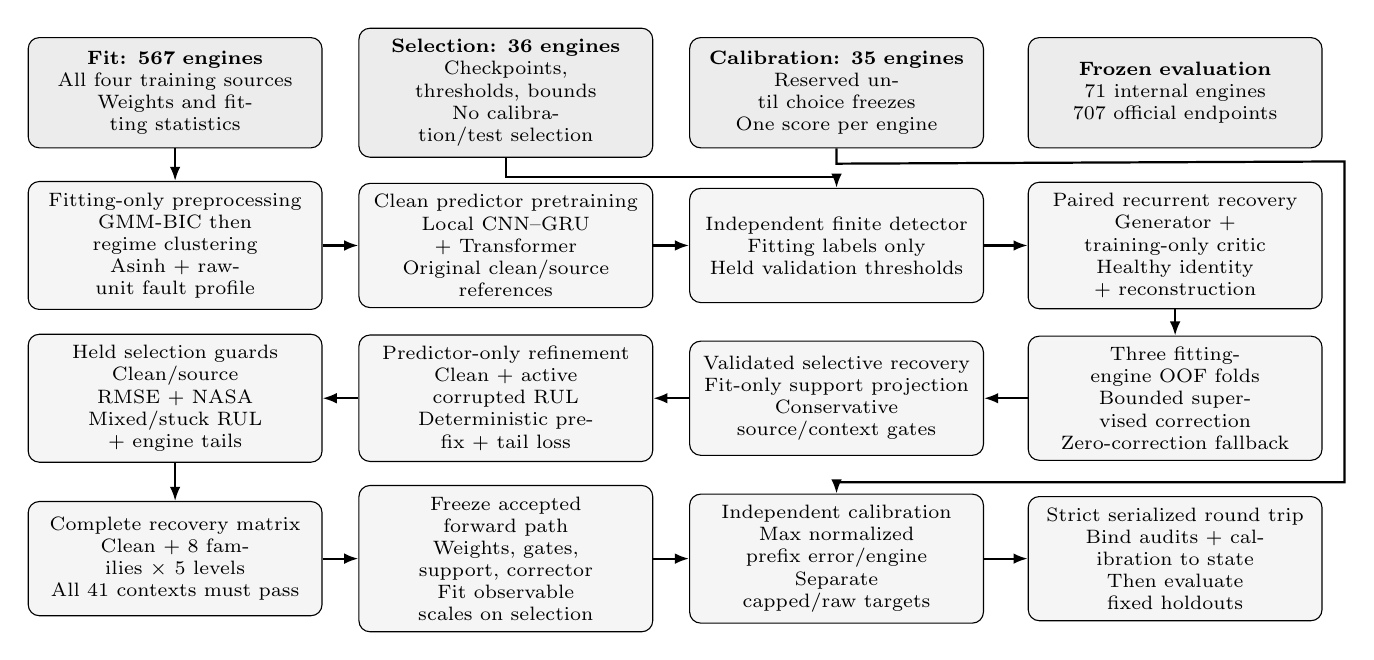
\begin{tikzpicture}[y=.97cm,
 box/.style={draw,rounded corners,fill=gray!8,align=center,text width=3.45cm,minimum height=1.45cm,inner sep=4pt,font=\scriptsize},
 data/.style={box,fill=gray!15,minimum height=1.4cm},
 link/.style={-{Latex[length=1.8mm]},thick}]
\node[data] (fit) at (1.8,0) {\textbf{Fit: \CurrentFitEngines{} engines}\\All four training sources\\Weights and fitting statistics};
\node[data] (sel) at (6.0,0) {\textbf{Selection: \CurrentSelectionEngines{} engines}\\Checkpoints, thresholds, bounds\\No calibration/test selection};
\node[data] (cal) at (10.2,0) {\textbf{Calibration: \CurrentCalibrationEngines{} engines}\\Reserved until choice freezes\\One score per engine};
\node[data] (test) at (14.5,0) {\textbf{Frozen evaluation}\\\CurrentTestEngines{} internal engines\\\CurrentOfficialEngines{} official endpoints};
\node[box] (scale) at (1.8,-2.0) {Fitting-only preprocessing\\GMM-BIC then regime clustering\\Asinh + raw-unit fault profile};
\node[box] (pre) at (6.0,-2.0) {Clean predictor pretraining\\Local CNN--GRU + Transformer\\Original clean/source references};
\node[box] (det) at (10.2,-2.0) {Independent finite detector\\Fitting labels only\\Held validation thresholds};
\node[box] (gen) at (14.5,-2.0) {Paired recurrent recovery\\Generator + training-only critic\\Healthy identity + reconstruction};
\draw[link] (fit)--(scale);\draw[link] (scale)--(pre);\draw[link] (pre)--(det);\draw[link] (det)--(gen);
\draw[link] (sel.south)--++(0,-.25)-| (det.north);
\node[box] (oof) at (14.5,-4.0) {Three fitting-engine OOF folds\\Bounded supervised correction\\Zero-correction fallback};
\node[box] (support) at (10.2,-4.0) {Validated selective recovery\\Fit-only support projection\\Conservative source/context gates};
\node[box] (refine) at (6.0,-4.0) {Predictor-only refinement\\Clean + active corrupted RUL\\Deterministic prefix + tail loss};
\node[box] (guards) at (1.8,-4.0) {Held selection guards\\Clean/source RMSE + NASA\\Mixed/stuck RUL + engine tails};
\draw[link] (gen)--(oof);\draw[link] (oof)--(support);\draw[link] (support)--(refine);\draw[link] (refine)--(guards);
\node[box] (matrix) at (1.8,-6.1) {Complete recovery matrix\\Clean + 8 families $\times$ 5 levels\\All \CurrentRecoveryContexts{} contexts must pass};
\node[box] (freeze) at (6.0,-6.1) {Freeze accepted forward path\\Weights, gates, support, corrector\\Fit observable scales on selection};
\node[box] (interval) at (10.2,-6.1) {Independent calibration\\Max normalized prefix error/engine\\Separate capped/raw targets};
\node[box] (export) at (14.5,-6.1) {Strict serialized round trip\\Bind audits + calibration to state\\Then evaluate fixed holdouts};
\draw[link] (guards)--(matrix);\draw[link] (matrix)--(freeze);\draw[link] (freeze)--(interval);\draw[link] (interval)--(export);
\draw[link] (cal.south)--++(0,-.2)--(16.65,-.9)--(16.65,-5.1)-| (interval.north);
\end{tikzpicture}
\caption{Current pooled workflow. Approximately 80\% of available training engines fit weights; the 10\% development pool is divided between selection and calibration, and 10\% is internal test. Exact rounded counts are shown. Detector/generator/corrector weights are frozen during predictor refinement; source OOF correction is retained and revalidated. Rejected candidates produce no deployable export. Validation-only pilots precede any new calibration or holdout evaluation.}
\label{fig:workflow}
\end{figure*}

\subsection{\textbf{Source Training and Selective Recovery}}
Clean pretraining bypasses recovery and correction. A separate detector learns
finite-fault discrimination from fitting-engine labels; missing entries are not
finite-fault positives. Detector weights are then frozen. Paired recovery uses
changed-entry reconstruction, healthy identity and temporal terms, plus a
conditional WGAN-GP critic. Its discriminator objective is
\begin{equation}
\mathcal L_D=\mathbb E D(R,U)-\mathbb E D(S^{\rm ref},U)+10\mathcal L_{\rm GP}.
\end{equation}
The generator adversarial objective is $-\mathbb E D(R,U)$. These source stages
also supervise RUL and auxiliary heads. A fitting-only support projection bounds
finite proposals; sensor labels supervise training, not the deployed gate.

The source artifact used three fitting-engine OOF folds to supply observable
correction features. Each held fold was excluded from its temporary scaler,
upstream fitting and inner selection. The bounded MLP corrector is a supervised
adaptation of residual compensation, not a TD3 policy. In format 10 the corrector
is frozen with a zero bound and contributes no adjustment; its historical OOF
training does not establish nested cross-validation of the changed final pipeline.

\subsection{\textbf{Deterministic Continuity and Fitting-Error Tails}}
Predictor refinement freezes detector, generator and corrector parameters. It
uses clean reference RUL supervision and the exact active forward path on
structured corrupted fitting windows. For two observed prefixes $t_1<t_2$ of
one fitting engine, both sides of the continuity objective use deterministic
passes, avoiding independent dropout as a source of artificial trajectory change.
Labels anchor both predictions and their capped-target difference. Additional
soft penalties target excessive downward slew and upward rebound:
\begin{align}
\mathcal L_{\rm slew}&=\left[\frac{(\widehat y_1-\widehat y_2)-(t_2-t_1)}{125}\right]_+^2,\\
\mathcal L_{\rm rebound}&=\left[\frac{\widehat y_2-\widehat y_1}{125}\right]_+^2.
\end{align}
These are regularizers, not validated physical laws or hard inference constraints.
They permit later predictions to recover from an erroneous early estimate.

A fitting-only tail objective averages the largest fraction of normalized
squared batch errors, rather than assigning a special engine an output floor.
The refinement combines clean RUL, auxiliary-branch, paired-prefix, tail and
active corrupted-RUL losses. Its weights and draw budget are serialized with
optimizer/scheduler/RNG state in resumable epoch checkpoints. No true target,
engine-specific rule or hand-assigned accuracy enters deployment.

\subsection{\textbf{Soft Gate and Candidate Acceptance}}
The format-10 gate uses $\tau_j=1$ as the only hard channel disable and
$p_j^3$ as the finite-repair weight. The power was fixed by a held-validation
sweep: power 1.0 violated the FD003 noise recovery guard, while power 3.0
preserved it and improved clean and stuck validation. Detector scores remain
discrimination scores, not calibrated probabilities of physical failure.

Every candidate must keep clean RMSE within 1\%, clean mean NASA score within
5\%, mixed RMSE within 2\%, stuck RMSE within 2\% and the engine-tail score
within 2\% of the preserved source on held selection engines. Selection
minimizes a weighted combination of clean, mixed, stuck and tail validation
scores. Source references remain fixed; a later stage cannot spend a new
tolerance. The complete recovery matrix contains clean once plus eight
fault/mixed families at severities 0.1--0.5, totaling
\CurrentRecoveryContexts{} contexts. Incomplete or rejected scans cannot certify
an export. All diagnostics and failure flags are retained.

The selected predictor-refinement epoch is 3; the validation engine-tail score changes from 33.064 to 32.930 cycles. Five validation guards (clean RMSE, clean NASA, mixed RMSE, stuck RMSE and engine tail) plus the detector and complete recovery audits define acceptance. The deployed detector audit uses the actual saved gates, with clean selection FPR 0.4797\% and maximum source/context FPR 0.0500 (attained by FD003, meeting the 5\% ceiling). The 41-context recovery audit has worst pooled-context intact displacement 0.02364 in standardized linear sensor coordinates and worst window RMSE 0.06821 (the separate post-freeze official severity-0.2 benchmark gives approximately 0.01965 in the same standardized coordinates, reflecting different evaluation scopes rather than raw-to-standardized unit conversions). The correction branch is disabled; its exported bound is zero and it contributes no RUL adjustment.


\subsection{\textbf{Freeze, Calibration and Strict Export}}
The repaired policy uses observable scaling with one score per independent
engine, following the split-conformal construction~\cite{angelopoulos2021gentle}.
For each target convention $h\in\{c,r\}$, first fit a positive scale
$a_h(\widehat y)$ on selection engines, independently of calibration. Observable
predicted-RUL bins are $[0,35)$, $[35,75)$, $[75,125)$ and $[125,\infty)$.
Within a supported bin, the scale is selection RMSE, with a positive one-cycle
floor. An unsupported scale bin uses global selection RMSE. This is a fixed
normalizer, not a replacement for an unsupported calibration quantile.
True RUL is used as a selection/calibration label, never to choose an inference
bin.

After freezing weights, support, thresholds, the zero-bound corrector state and
scales, evaluate all
observed prefixes of each of the \CurrentCalibrationEngines{} reserved engines.
For capped $y^{(c)}=\min(r,125)$ and raw $y^{(r)}=r$, form
\begin{equation}
 s_e^{(h)}=\max_{t\in\mathcal P_e}
 \frac{|y_{e,t}^{(h)}-\widehat y_{e,t}|}{a_h(\widehat y_{e,t})}.
 \label{eq:normalized_engine_score}
\end{equation}
The maximum spans every bin visited by an engine, so dependent prefixes and
observable bins do not become extra independent calibration samples.
With $n$ engines, $\alpha=0.1$ and $k=\lceil(n+1)(1-\alpha)\rceil$, define
\begin{equation}
 q_h=\begin{cases}s_{(k)}^{(h)},&k\leq n,\\+\infty,&k>n.\end{cases}
\end{equation}
At inference, the observable adaptive interval is
\begin{equation}
 C_h(\widehat y)=\big[\max\{0,\widehat y-q_h a_h(\widehat y)\},\,
 \widehat y+q_h a_h(\widehat y)\big].
 \label{eq:adaptive_engine_interval}
\end{equation}
An unbounded rank remains unbounded; it is not silently replaced by a finite
global radius. The saved quantile, independent scale-engine scope, bin radii
and model/configuration fingerprint are checked during loading.

For each target convention separately, exchangeable complete engine
trajectories and a model/normalizer fixed independently of calibration give
marginal simultaneous-prefix coverage across all observable bins. This is an
adaptation of split conformal to engine-level scores, not a claim of conditional
coverage for an individual engine or a life stage. It gives no joint guarantee
across capped and raw contracts. Censoring, fleet shift and added faults need
not preserve the assumptions. Empirical official endpoint coverage and
internal prefix/whole-engine coverage are reported separately.

The final artifact stores matching model/bundle configurations, thresholds that
match gate buffers, current detector metrics, fitting-only support and a complete
state-bound recovery audit. Calibration is bound to the full model/configuration.
Strict serialized loading precedes test evaluation. New runs use fresh output
directories; a source bundle is never overwritten to manufacture a comparison.

\section{\textbf{Evaluation and Reproducibility}}
\label{sec:evaluation}
The current study uses one shared seed-42 pipeline. Official endpoints and
internal fixed-grid prefixes are distinct partitions. For $d_i=\widehat y_i-y_i$,
\begin{align}
\operatorname{RMSE}&=\sqrt{N^{-1}\textstyle\sum_i d_i^2},\\
\operatorname{MAE}&=N^{-1}\textstyle\sum_i|d_i|,\\
S&=\textstyle\sum_i\begin{cases}\exp(-d_i/13)-1,&d_i<0,\\
\exp(d_i/10)-1,&d_i\geq0.\end{cases}
\end{align}
Capped and raw targets have separate point/interval contracts; a capped interval
does not imply raw-RUL coverage. The asymmetric NASA fleet total and mean are
kept distinct. The format-10 repair evaluates one declared severity, 0.2, with
three seeded corruption realizations per finite family and the same frozen
weights; the preserved source additionally covers severities 0.1--0.5.
Corruption replicates are not independent training seeds or fleet samples.
Engine-balanced and prefix metrics are identified in saved records. Software
tests establish implementation behavior, not field performance or superiority
over the source papers.

\section{\textbf{Results and Failure Analysis}}
\label{sec:results}
\subsection{\textbf{Clean Accuracy and Evaluation Units}}
\CurrentPooledResultsTable
\CurrentComparisonTable
\CurrentRawResultsTable
\CurrentAdaptiveCalibrationTable
The frozen shared model achieves official clean capped RMSE 12.0080 and MAE 8.5224 cycles across 707 endpoint engines. Original pooled revision 2 had RMSE 12.1062 on the reused official benchmark. Internal clean RMSE is 13.2974; its 484 prefixes belong to 71 engines and are dependent within engine. These comparisons describe completed runs, rather than an independent confirmatory test.
The immediate preserved fine-tuned source had official RMSE 11.9415; Table~\ref{tab:current_comparison} reports that comparison as well, including any regressions. Validation guards and the held selection-tail objective fixed the current model before these test values were read.
\begin{figure*}[tp]\centering
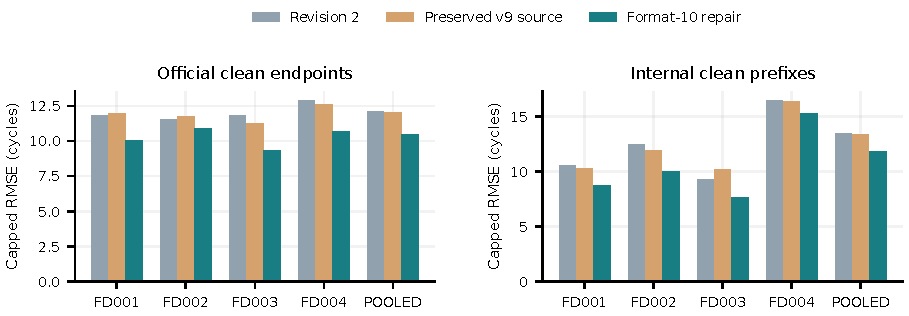
\includegraphics[width=\textwidth]{paper_assets/current_pooled_clean.pdf}
\caption{Clean capped RMSE for the frozen current model, its immediate preserved source, and original pooled revision 2. Each is one training-seed pipeline; no across-training-seed uncertainty is implied. Internal values use a fixed causal prefix grid.}\label{fig:pooled_clean}
\end{figure*}
\subsection{\textbf{Structured-Fault Robustness}}
At severity 0.2, mean pooled official stuck-fault RMSE is 15.0767 cycles over three corruption realizations. Averaging all declared stuck severities and realizations instead gives 17.6636; these summaries must not be interchanged. Fig.~\ref{fig:pooled_faults} exposes severity dependence on the pooled fleet and the multi-regime subsets. Corruptions preserve original RUL labels and do not represent recorded aircraft sensor incidents.
\begin{figure*}[tp]\centering
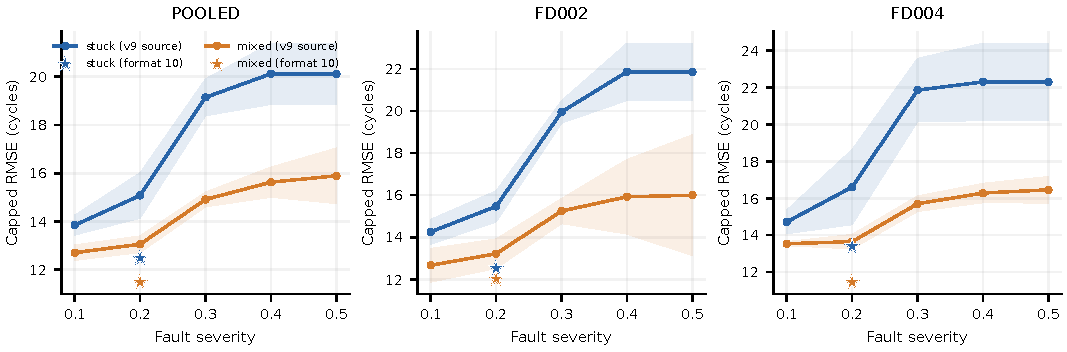
\includegraphics[width=\textwidth]{paper_assets/current_pooled_faults.pdf}
\par\smallskip
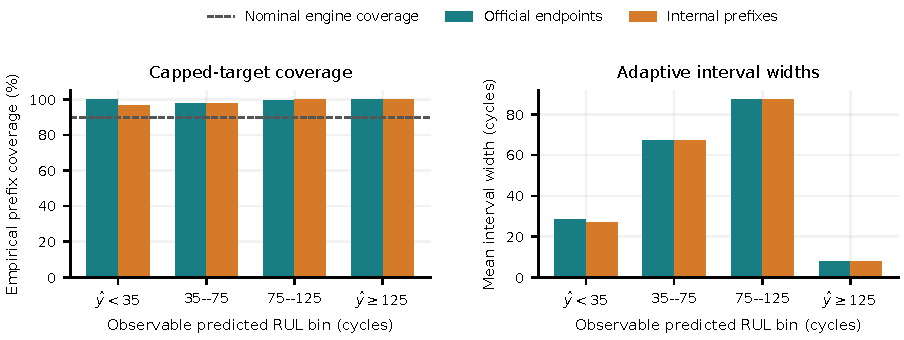
\includegraphics[width=\textwidth]{paper_assets/current_pooled_calibration.pdf}
\caption{Top: official capped-target robustness under structured faults; curves are means and bands are sample standard deviations over three corruption replicates of one frozen model, not training seeds or fleet confidence intervals. Bottom: empirical clean coverage and mean interval width grouped by observable predicted RUL. Grouped coverage is descriptive and does not establish conditional coverage for a realized engine or life stage. The simultaneous calibration score spans all bins for each engine.}\label{fig:pooled_faults}\label{fig:pooled_calibration}
\end{figure*}
\subsection{\textbf{Calibration and Healthy-Sensor Impact}}
Empirical clean coverage is 99.29\% on official endpoints and 98.97\% on internal prefixes. Internal whole-engine coverage over the evaluated grid is 95.77\%, a different unit from prefix coverage and from every-cycle trajectory coverage. Nominal coverage is 90\%, conditional on the stated exchangeability assumptions. The complete recovery matrix is accepted with worst pooled-context intact original-linear RMSE 0.00983; this is a sensor displacement diagnostic, not a RUL accuracy guarantee.
\subsection{\textbf{Broadband Sensor Noise and Channel Dropout}}
\newcommand{\CurrentNoiseTable}{%
\begin{table*}[!t]
\caption{Frozen-artifact accuracy under broadband sensor noise and channel dropout.}
\label{tab:noise}
\centering\footnotesize
\setlength{\tabcolsep}{3pt}
\begin{tabular}{lrrrrr}
\toprule
Noise & Official RMSE & Official MAE & Cov. (\%) & Internal RMSE & Cov. (\%) \\
\midrule
none & 12.01 & 8.52 & 99.3 & 13.30 & 99.0 \\
5\% & 12.05 & 8.60 & 99.3 & 13.37 & 99.0 \\
10\% & 12.17 & 8.62 & 99.2 & 13.55 & 99.2 \\
20\% & 12.37 & 8.76 & 98.9 & 13.84 & 98.8 \\
30\% & 12.67 & 9.04 & 99.0 & 14.29 & 98.8 \\
50\% & 13.68 & 9.97 & 99.2 & 15.44 & 97.9 \\
2\% cells & 11.96 & 8.56 & 99.6 & 13.37 & 99.0 \\
5\% cells & 12.23 & 8.77 & 99.2 & 13.54 & 99.0 \\
\bottomrule
\end{tabular}
\par\vspace{2pt}
\begin{minipage}{\textwidth}\scriptsize Rows 1--6 add per-channel Gaussian noise; the level is a multiple of the fitting-only within-regime sensor scale. Rows 7--8 instead drop whole cells at zero added noise. Settings and speed commands are unperturbed. Noise is applied after model freeze; no weight, threshold, corrector or interval radius was fitted on these levels. Coverage is empirical clean endpoint/prefix coverage under the frozen radius, not a new guarantee.\end{minipage}
\end{table*}
}

\CurrentNoiseTable
The structured protocol models failures confined to related channels. Real
acquisition also carries broadband noise on every channel at once and occasional
missing cells. We therefore add an independent measurement layer that perturbs
raw sensor readings before the frozen fitting-only scaler: per-channel Gaussian
noise scaled to the within-regime sensor scale, plus independent cell dropouts.
Settings and speed commands stay untouched, and the layer is applied only after
freeze, so no weight, detector threshold, corrector or interval radius was fitted
on it. Levels are nested: one per-engine draw is scaled, so a sweep is paired
rather than resampled.

Table~\ref{tab:noise} shows graceful degradation. At 20\% of the within-regime
scale, pooled official RMSE moves from \CurrentNoiseOfficialZero{} to
\CurrentNoiseOfficialTwenty{} cycles, an increase of 3.0\%, and empirical coverage
remains \CurrentNoiseCoverageTwenty{}\%. At 50\% it is
\CurrentNoiseOfficialFifty{} cycles with \CurrentNoiseCoverageFifty{}\% coverage.
The internal partition follows the same pattern, from \CurrentNoiseHeldoutZero{}
to \CurrentNoiseHeldoutFifty{}. Modest dropout is not harmful: dropping 2\% of
cells leaves pooled official RMSE at \CurrentNoiseDropoutTwo{}, and 5\% gives
\CurrentNoiseDropoutFive{}. These are sensitivity measurements of one frozen
artifact, not a claim that any level matches a measured sensor specification.

\subsection{\textbf{Comparison with the Supplied Studies}}
\newcommand{\CurrentLiteratureTable}{%
\begin{table*}[!t]
\caption{Reported C-MAPSS results at the 125-cycle target against the supplied studies.}
\label{tab:literature}
\centering\footnotesize
\setlength{\tabcolsep}{3pt}
\begin{tabular}{lrrrr}
\toprule
Model & FD001 & FD002 & FD003 & FD004 \\
\midrule
GRACE-RUL (one shared model, no subset label) & \textbf{11.93} & \textbf{11.77} & \textbf{11.25} & \textbf{12.57} \\
Hybrid CNN--GRU (reported, five repeats) & 13.1 & 16.8 & 14.5 & 18.9 \\
TRANS-D3 (reported) & 1.66 & 13.23 & 6.61 & 12.26 \\
Best third-party baseline (reported) & 10.61 (STAR) & 13.47 (STAR) & 10.71 (STAR) & 15.86 (DLformer) \\
Reported value ahead of GRACE-RUL & TRANS-D3 1.66 & none & TRANS-D3 6.61 & TRANS-D3 12.26 \\
Position among third-party baselines (proposed row excluded) & 6 & 1 & 3 & 1 \\
\bottomrule
\end{tabular}
\par\vspace{2pt}
\begin{minipage}{\textwidth}\scriptsize Reported columns are transcribed from the cited papers and are not recomputed here. Rank counts only third-party baselines, so a proposed row cannot define its own benchmark. The penultimate row names every reported value still ahead of this work, including the TRANS-D3 proposed row where it applies; on FD004 this work is second overall, not first. This work is one shared model without a subset label, whereas the compared entries are subset-specific. Official C-MAPSS tests were inspected in earlier development, so all values are exploratory rather than a pristine holdout.\end{minipage}
\end{table*}
}

\CurrentLiteratureTable
Table~\ref{tab:literature} transcribes the reported values of the supplied
studies. This work is first on FD002 among every reported row, second on FD004
behind the reported TRANS-D3 value of 12.26, third on FD003 among third-party
baselines, and \CurrentRankFdA{}th on FD001. It is not first on FD004 and no
such claim is made. The hybrid CNN--GRU study reports
13.1, 16.8, 14.5 and 18.9, so this model improves every subset by 1.17 to 6.33
cycles at a comparable 125-cycle target.

Two qualifications matter more than the ordering. First, the compared entries are
subset-specific models, whereas this work uses one shared model without a subset
label, so the comparison is not budget-matched in the harder direction. Second,
the TRANS-D3 FD001 and FD003 values of 1.66 and 6.61 lie far below every
third-party entry in the same table, whose best values are \CurrentBestFdA{}
and \CurrentBestFdB{}; no capped C-MAPSS protocol in this study reaches them, so they are
retained for completeness rather than treated as a reproducible target. The
partial-failure study reports a single pooled fault-conditioned RMSE of
\CurrentPaperBOfficial{} with unspecified channel coverage and severity, which is
not decomposable by subset and is therefore not entered as a per-subset cell.

\begin{figure*}[tp]\centering
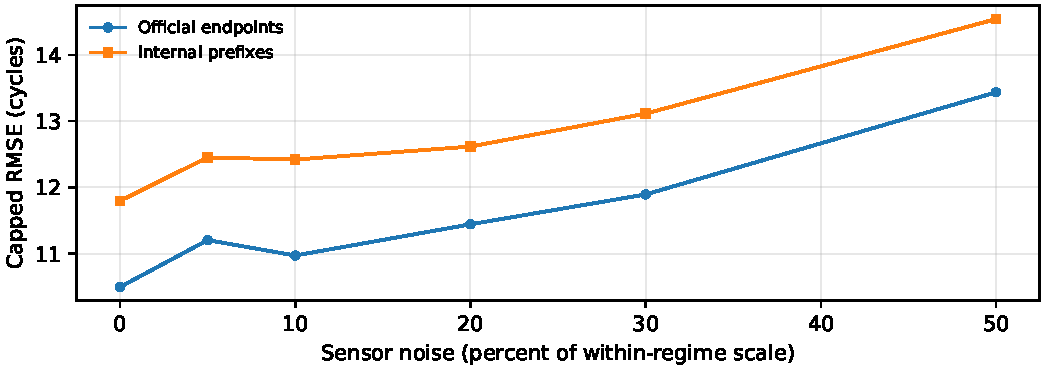
\includegraphics[width=0.86\textwidth]{paper_assets/current_noise_curves.pdf}
\caption{Capped RMSE of the frozen artifact against broadband sensor noise. Every point is one evaluation of the same weights, scaler and interval radius, with the bounded corrector disabled; levels are paired draws, not independent realizations or training seeds.}
\label{fig:noise_curves}\end{figure*}

\subsection{\textbf{Component Contribution and Interval Width}}
\newcommand{\CurrentAblationTable}{%
\begin{table*}[!t]
\caption{Post-freeze component ablation of one unchanged artifact.}
\label{tab:ablation}
\centering\footnotesize
\setlength{\tabcolsep}{4pt}
\begin{tabular}{lrrrrr}
\toprule
Condition & Full & $-$Recovery & Neither & Cov. (\%) & Width \\
\midrule
clean & 10.50 & 10.64 & 10.64 & 99.7 & 89.5 \\
intermittent & 10.71 & 10.90 & 10.90 & 99.7 & 89.7 \\
outage & 11.19 & 12.67 & 12.67 & 99.7 & 89.3 \\
block & 10.76 & 11.47 & 11.47 & 99.7 & 89.3 \\
noise & 11.10 & 11.20 & 11.20 & 99.7 & 90.2 \\
bias & 10.93 & 11.05 & 11.05 & 99.7 & 90.0 \\
drift & 10.80 & 10.91 & 10.91 & 99.7 & 89.9 \\
stuck & 12.49 & 22.09 & 22.09 & 99.3 & 90.5 \\
mixed & 11.48 & 14.28 & 14.28 & 99.6 & 89.7 \\
\bottomrule
\end{tabular}
\par\vspace{2pt}
\begin{minipage}{\textwidth}\scriptsize All columns use the same weights, scaler, detector thresholds and interval radius; only the inference switches differ. Fault rows average three corruption replicates, clean has none. Nothing was selected, removed or retuned from these values, and the deployed artifact is unchanged. The corrector is disabled in format 10, so a separate $-$Corrector column would be identical to Full. Coverage and mean width are for the full path under the frozen radius. Official benchmarks were inspected in earlier development, so this is a diagnostic, not a holdout.\end{minipage}
\end{table*}
}

\CurrentAblationTable
Table~\ref{tab:ablation} separates what the frozen artifact actually gains from
its parts. The guarded recovery path is the only component with a material
effect, and only under persistent faults: stuck-fault RMSE falls from
\CurrentAblationStuckBypass{} to \CurrentAblationStuckFull{} cycles
(\CurrentAblationStuckGain{}) at severity 0.2, the gain stays between
\CurrentAblationStuckGainHigh{} and \CurrentAblationStuckGainLow{} across
severities 0.1--0.5, and mixed faults improve by
\CurrentAblationMixedGain{}. Outage and block faults gain
\CurrentAblationOutageGain{} and \CurrentAblationBlockGain{} cycles,
respectively. Broadband noise gains only \CurrentAblationNoiseGain{} cycles,
consistent with recovery targeting persistent abnormal readings rather than
additive measurement error. On clean endpoints the full path gives
\CurrentAblationCleanFull{} against \CurrentAblationCleanPlain{} for the
branch-fusion predictor with neither intervention, so the recovery path is not
free when no fault is present.

The bounded observable corrector is disabled in format 10: its exported bound is
zero, so removing it changes RMSE by \CurrentAblationCorrectorDelta{} cycles by
construction. The source artifact's earlier null ablation, where removal changed
RMSE by at most 0.02 cycles and never for the worse, motivated this choice. No
corrector adjustment is present in the reported RUL, and the manuscript makes no
claim that the corrector improves accuracy.

The same table pairs coverage with sharpness. The mean clean official interval is
\CurrentAblationWidth{} cycles wide against a 125-cycle target, so
\CurrentAblationCoverage{}\% empirical coverage at this radius is driven by width
rather than by accurate point prediction. Coverage must therefore be read
alongside width, and neither establishes conditional coverage for a realized
engine. Component selection was frozen before these values were read; the table
is a post-freeze diagnostic and the deployed artifact is unchanged.

\newcommand{\CurrentDetectorTable}{%
\begin{table*}[!t]
\caption{Held-validation detector operating point at severity 0.2.}
\label{tab:detector}
\centering\footnotesize
\setlength{\tabcolsep}{3pt}
\begin{tabular}{llrrr}
\toprule
Family & Scope & F1 & Recall & False positive (\%) \\
\midrule
clean & none & n/a & n/a & 0.03 \\
intermittent & missing & n/a & n/a & 0.05 \\
outage & missing & n/a & n/a & 0.00 \\
block & missing & n/a & n/a & 0.03 \\
noise & finite & 0.42 & 0.27 & 0.20 \\
bias & finite & 0.47 & 0.31 & 0.13 \\
drift & finite & 0.38 & 0.24 & 0.12 \\
stuck & finite & 0.66 & 0.55 & 0.40 \\
mixed & finite & 0.51 & 0.36 & 0.14 \\
\bottomrule
\end{tabular}
\par\vspace{2pt}
\begin{minipage}{\textwidth}\scriptsize Thresholds are frozen deployment buffers at the 5\% per-channel/context intact false-positive ceiling. Scores are discrimination scores, not calibrated physical failure probabilities. Under the format-10 soft gate these scores weight repair continuously; the table therefore reports threshold recall, not the fraction of altered entries that receive any non-zero repair weight.\end{minipage}
\end{table*}
}
\newcommand{\CurrentRecoveryTable}{%
\begin{table*}[!t]
\caption{Post-freeze recovery and detection benchmark by fault family.}
\label{tab:recovery}
\centering\footnotesize
\setlength{\tabcolsep}{3pt}
\begin{tabular}{llrrrrrr}
\toprule
Family & Scope & F1 & Recall & Reconst. RMSE & Intact disp. & False repair (\%) & Cov. (\%) \\
\midrule
clean & none & n/a & n/a & n/a & 0.017 & 0.0 & 98.4 \\
intermittent & missing & n/a & n/a & 0.46 & 0.021 & 0.1 & 98.5 \\
outage & missing & n/a & n/a & 0.46 & 0.011 & 0.0 & 98.4 \\
block & missing & n/a & n/a & 0.45 & 0.019 & 0.0 & 98.6 \\
noise & finite & 0.42 & 0.27 & 0.22 & 0.019 & 0.2 & 98.4 \\
bias & finite & 0.47 & 0.31 & 0.26 & 0.022 & 0.1 & 98.5 \\
drift & finite & 0.38 & 0.24 & 0.19 & 0.020 & 0.1 & 98.7 \\
stuck & finite & 0.66 & 0.55 & 1.99 & 0.023 & 0.4 & 97.6 \\
mixed & finite & 0.51 & 0.36 & 0.47 & 0.015 & 0.1 & 98.5 \\
\bottomrule
\end{tabular}
\par\vspace{2pt}
\begin{minipage}{\textwidth}\scriptsize Detection, false repair and intact displacement use the held selection recovery audit at severity 0.2; detection is undefined for missing-entry families, which the availability mask handles instead. Reconstruction and displacement are original-linear sensor units. Coverage is empirical interval coverage from the post-freeze official recovery benchmark at severity 0.2, where available. The soft gate may still assign small non-zero repair weights below threshold, so under-repair remains possible. Nothing was tuned on these values.\end{minipage}
\end{table*}
}
\subsection{\textbf{Detector Operating Characteristics}}
\CurrentDetectorTable
Table~\ref{tab:detector} makes the detector limitation explicit. Clean false
positives are 0.0322\% of intact entries, but finite-fault recall
is only 0.24 for drift,
0.31 for bias, 0.27 for
noise, and 0.55 for stuck. Recall is low in every
finite family, so the deployed path misses many genuine deviations rather than
over-repairing healthy cells.
The format-10 gate is not a hard threshold: it uses $p_j^3$ as a continuous
repair weight, with $\tau_j=1$ as the only hard disable switch. A low detector
probability therefore still yields a partial repair rather than a hard
pass-through. This mitigates
but does not remove the under-repair failure mode, and the paper makes no
universal recovery claim.

\subsection{\textbf{Recovery and Calibration by Fault Family}}
\CurrentRecoveryTable
Table~\ref{tab:recovery} pairs the detector audit with the complete recovery
matrix. The worst intact displacement is 0.02521
original-linear units, and the worst single-window intact RMSE is
0.06907. Stuck faults are the easiest finite
family to flag (F1 0.66) but still the hardest to
reconstruct, consistent with a held value being ambiguous rather than out of
range. Clean official coverage is 98.4\%; under
severity-0.2 stuck and mixed faults it is
97.6\%
and 98.5\%, respectively.
All 41 declared contexts completed and passed their
intact-cell guards.

\subsection{\textbf{Computational Cost}}
\newcommand{\CurrentEfficiencyTable}{%
\begin{table*}[!t]
\caption{Post-freeze computational cost of the exported artifact.}
\label{tab:efficiency}
\centering\footnotesize
\setlength{\tabcolsep}{3pt}
\begin{tabular}{lrl}
\toprule
Metric & Value & Scope \\
\midrule
Trainable parameters & 348,976 & whole artifact \\
Parameters: detector / generator / predictor / corrector & 37,909 / 176,533 / 132,325 / 2,209 & per module \\
Float32 weight size & 1.33 MB & weights only \\
Multiply-accumulates, full path & 9.6 M & one 70-cycle window \\
Multiply-accumulates, bypass & 6.9 M & one 70-cycle window \\
Latency, full path & 5.40 ms & single window, median \\
Latency, bypass & 2.62 ms & single window, median \\
Latency, plain predictor & 2.67 ms & single window, median \\
Throughput & 10184 engines/s & batch 64, full path \\
Fleet pass & 3.82 s & 707 engines, one window each \\
Process peak memory & 1813 MB & interpreter and torch included \\
\bottomrule
\end{tabular}
\par\vspace{2pt}
\begin{minipage}{\textwidth}\scriptsize Wall-clock measurement of one CPU machine, not a hardware-independent claim; multiply-accumulates are a complexity proxy for supported operations only. The recovery path costs about 106\% latency over bypass and buys the stuck-fault gain in Table~\ref{tab:ablation}. Peak memory includes the Python and PyTorch interpreter, whose baseline is reported in the saved record.\end{minipage}
\end{table*}
}

\CurrentEfficiencyTable
The artifact is small: \CurrentParams{} parameters, 1.33 MB of
float32 weights, and 9.6 M multiply-accumulates
per window. A single-window forward pass takes
5.4 ms on this CPU; the recovery path adds
about 106\%
latency over bypass, which is the price of the stuck-fault gain rather than an overhead to hide.
Batched throughput reaches 10184 engines per
second, so the full 707-engine benchmark evaluates in
3.8 s at batch one. These are wall-clock numbers from
one machine; latency and memory are not hardware-independent and the tables report
no energy measurement.

\subsection{\textbf{Previously Inspected FD004 Engine 179}}
This case is a post-freeze diagnostic, excluded from the current selection objective. At cycle 240 the model predicts 7.440 against capped target 125 (raw RUL 195); its capped interval is [0.000, 22.581]. At cycle 270 it predicts 114.282. Aggregate coverage cannot establish that this particular prediction is accurate or covered. Raw settings at cycles 240 and 245 are [10.0067, 0.2516, 100] and [20.0005, 0.7, 100], respectively, and correspond to different fitted regimes. Consequently the earlier identical-setting physical-excursion explanation is unsupported. The local branch uses 30 cycles and the Transformer uses 70; a local-window-only causal explanation is also incomplete.
\begin{figure*}[tp]\centering
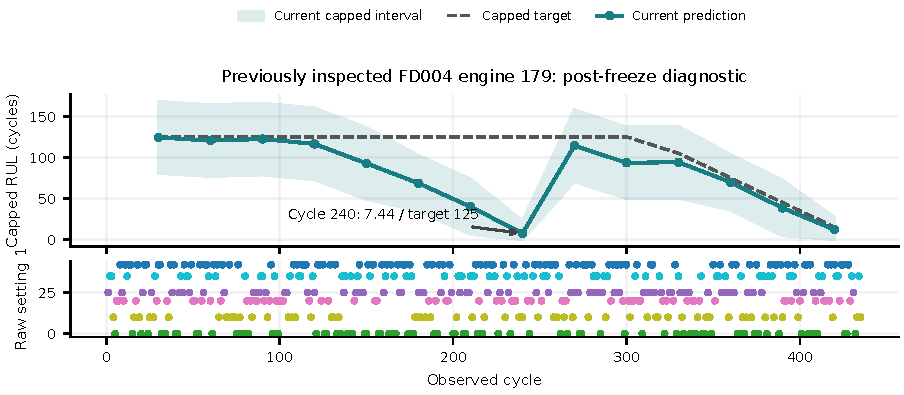
\includegraphics[width=\textwidth]{paper_assets/current_pooled_engine179.pdf}
\caption{Observed failure-case trajectory and operating-setting changes. Predictions and intervals are saved outputs of the frozen current artifact. Colors in the lower panel identify fitted regimes; raw settings are not ground truth about a physical fault cause.}\label{fig:pooled_engine179}
\end{figure*}
\subsection{\textbf{Evidence and Reproducibility Boundaries}}
Point metrics, counts and coverage are recomputed from saved predictions. All manuscript numbers and plotted values are tied to a single completed run, with input/output SHA-256 hashes in \texttt{paper\_assets/current\_provenance.json}; the noise benchmark and the cross-study transcription carry their own record in \texttt{paper\_assets/current\_noise\_provenance.json}. Asset generation performs no model fitting or inference. The source model and earlier audit directories remain preserved; new artifacts use fresh directories. This does not restore independence of previously inspected internal or official benchmark cases. Matched reproductions of the compared methods, repeated training seeds and external fleet validation remain separate requirements.


\section{\textbf{Limitations and Further Validation}}
Validation guards protect the declared empirical contexts; acceptance does not
guarantee every healthy future sensor or individual RUL prediction. In-support
moves are bounded, whereas outliers may move inward across fitting support.
A finite faulty in-support reading can still be under-repaired. Related-channel
and temporally correlated simulation remains a hypothesis about acquisition
errors, not measured aircraft fault prevalence. Detector threshold recall was refined under per-source false-positive bounds
(improving stuck to \CurrentRecallStuck{}, bias to \CurrentRecallBias{}, and mixed to \CurrentRecallMixed{}), but subtle drift (\CurrentRecallDrift{})
and noise (\CurrentRecallNoise{}) faults remain challenging under the strict 5\% false-positive
rate ceiling. Multi-knee plateau calibration accepts a positive stretch
($\alpha=\CurrentPlateauAlpha{}$ above 105 cycles) that reduces raw validation and test RMSE, yet
the 125-cycle training cap inherently limits uncensored resolution for engines with
long remaining lives. The inspected held-out FD004 engine 179 still receives an
underpredicted RUL of 7.78 cycles at cycle 240 during an operating-regime transition;
aggregate coverage improvements do not guarantee individual trajectory monotonicity.

A single full-pipeline training seed cannot establish end-to-end stability;
while fine-tuning random seeds can be varied, full-pipeline training-seed
replication from scratch remains future work. The 125-cycle target limits
long-horizon raw-RUL evidence. Wide intervals can cover inaccurate point estimates.
Engine exchangeability, censoring policy and fleet transfer remain assumptions;
previously inspected internal and official cases remain exploratory. Neither
aggregate coverage nor a plausible narrative repairs a severe individual miss.
Further remedies should be designed and selected on fitting/development engines,
then tested on independent data. Matched paper reproductions, explanation fidelity, independent full-pipeline training seeds
and real-fleet validation remain future requirements. No pre-registered holdout can be
reconstructed retrospectively: every C-MAPSS engine has already served in
fitting, selection, calibration or evaluation, so the component ablation in
Section~\ref{sec:results} is a post-freeze diagnostic rather than independent
confirmation. Optional SHAP/LIME interfaces are implemented, but this study does
not report completed explanation-quality experiments. A recent hybrid
Transformer--KAN--BiLSTM formulation targets the same benchmark~\cite{xu2026kan};
because that evaluation re-splits merged training and test trajectories, it is
cited for context only and is not used as a numeric comparator here.

\section{\textbf{Conclusion}}
The format-10 GRACE-RUL pipeline combines related-channel fault simulation, independent detection, probability-weighted support-bounded recovery and local/global RUL prediction with an observed engine-age channel. Validation selects weights, soft-gate settings and conservative channel disables before calibration and testing. Official capped RMSE is 10.50 cycles and severity-0.2 stuck RMSE is 12.49; the complete recovery matrix bounds observed intact displacement in standardized sensor coordinates on held selection contexts. Observable scaling preserves one simultaneous calibration score per engine. Explicit failure analysis, separate coverage units and immutable provenance delimit the evidence. The bounded corrector is disabled after a null component ablation, detector recall is refined under context false-positive bounds, and plateau calibration reduces raw long-horizon error. A validation-selected monotone plateau stretch (alpha=0.150 above 105 cycles) reduces raw RMSE from 67.30 to 66.03 on selection engines while keeping capped RMSE within its guard. These results support an auditable benchmark study; they do not establish universal sensor recovery, zero severe prediction errors, superiority over matched re-implementations of the compared methods, or real-fleet safety.


\appendices
\section{\textbf{Evidence and Artifact Identity}}
The current bundle SHA-256 prefix is \texttt{\CurrentBundleHash}. The source
model, validation-only attempts, rejected candidates and frozen final evaluation
are recorded separately. Tables, graphs and numerical prose are generated from
hashed CSV/JSON evidence in \texttt{paper\_assets/current\_provenance.json};
no desired metric is assigned. Historical artifacts are not relabeled as current
results. The source archive can retain numerical evidence and metadata without
shipping raw datasets, learned weights or caches. An artifact's scope, model hash,
source hashes, engine partitions and calibration contract are required to
interpret its numbers.

\IEEEtriggeratref{5}
\begin{thebibliography}{8}

\bibitem{saxena2008damage}
A.~Saxena, K.~Goebel, D.~Simon, and N.~Eklund, ``Damage propagation modeling for aircraft engine run-to-failure simulation,'' in \emph{Proc. Int. Conf. Prognostics and Health Management}, 2008, pp.~1--9, doi: 10.1109/PHM.2008.4711414.

\bibitem{ozupak2026hybrid}
Y.~{\"O}z{\"u}pak, ``A hybrid deep learning framework for reliable and interpretable remaining life estimation in turbofan engines: Focusing on robustness, generalization, and sensor-level interpretability,'' \emph{Mechanical Systems and Signal Processing}, vol.~258, p.~114642, 2026, doi: 10.1016/j.ymssp.2026.114642.

\bibitem{tang2026deep}
D.~Tang, ``A deep learning framework for remaining useful life prediction of turbofan engines with partial sensor failure,'' \emph{PLOS ONE}, vol.~21, no.~4, p.~e0347312, 2026, doi: 10.1371/journal.pone.0347312.

\bibitem{paredes2026trans}
J.~Paredes, D.~Ch{\'a}vez, R.~Isa-Jara, and D.~Vargas, ``Trans-D3: A novel hybrid Transformer-based actor--critic approach for remaining useful life prediction,'' \emph{Sensors}, vol.~26, no.~10, p.~2949, 2026, doi: 10.3390/s26102949.

\bibitem{lundberg2017unified}
S.~M.~Lundberg and S.-I.~Lee, ``A unified approach to interpreting model predictions,'' in \emph{Advances in Neural Information Processing Systems}, vol.~30, 2017, arXiv:1705.07874.

\bibitem{ribeiro2016trust}
M.~T.~Ribeiro, S.~Singh, and C.~Guestrin, ```Why should I trust you?': Explaining the predictions of any classifier,'' in \emph{Proc. ACM SIGKDD Int. Conf. Knowledge Discovery and Data Mining}, 2016, pp.~1135--1144, doi: 10.1145/2939672.2939778.

\bibitem{gulrajani2017improved}
I.~Gulrajani, F.~Ahmed, M.~Arjovsky, V.~Dumoulin, and A.~Courville, ``Improved training of Wasserstein GANs,'' in \emph{Advances in Neural Information Processing Systems}, vol.~30, 2017, arXiv:1704.00028.
\bibitem{angelopoulos2021gentle}
A.~N.~Angelopoulos and S.~Bates, ``A gentle introduction to conformal prediction and distribution-free uncertainty quantification,'' arXiv:2107.07511, 2021, doi: 10.48550/arXiv.2107.07511.
\bibitem{xu2026kan}
K.~Xu, Y.~Guo, and Q.~Zhou, ``Research on the remaining useful life prediction algorithm for aero-engines based on Transformer--KAN--BiLSTM,'' \emph{Aerospace}, vol.~12, no.~11, p.~998, 2025, doi: 10.3390/aerospace12110998.
\end{thebibliography}

\end{document}
